\documentclass[a4paper,11pt,bibliography=totoc,listof=totoc,headinclude=true,cleardoublepage=empty,oneside]{scrbook}
% Option "oneside" für einseitigen Druck. Weglassen, falls die Arbeit doppelseitig gedruckt wird

\usepackage[english]{babel}
\usepackage[utf8]{inputenc}
%\usepackage{fullpage}
\usepackage{ifthen}
\usepackage{color}
\usepackage{amsmath,amsthm,amssymb,amsfonts}
\usepackage{graphicx}
\usepackage{psfrag}
\usepackage{epstopdf}

% links in pdf
\usepackage[unicode,colorlinks=true,pagebackref=false]{hyperref}

% Zum Druck verwende schwarze Links!
%\usepackage[unicode,colorlinks=true,linkcolor=black,citecolor=black,urlcolor=black,pagebackref=false]{hyperref} 
	% colorlinks=false umrahmt Links statt einzufaerben, 


\usepackage{amsmath}
\usepackage{amssymb}
\usepackage{amsthm}
\usepackage{bbm}
\usepackage{enumerate}
\usepackage{epstopdf}
\usepackage[shortlabels]{enumitem}
\usepackage{algorithm}
\usepackage{algpseudocode}
\usepackage{graphicx}
\usepackage{subcaption}

\newtheorem{definition}{Definition}
\newtheorem{lemma}{Lemma}
\newtheorem{theorem}{Theorem}


% document style
\KOMAoptions{footinclude=false} % Fusszeile wird nicht zu Satzspiegel gezaehlt
\KOMAoptions{headsepline=true} % Trennlinie zwischen Kopfzeile und Text
\KOMAoptions{DIV=12} % beeinflusst Satzspiegel
\KOMAoptions{BCOR=8mm} % Bindekorrektur
\pagestyle{headings} % mit Kopfzeilen

\recalctypearea % berechne Satzspiegel neu

\definecolor{change}{rgb}{0,.55,.55}

\def\revision#1{{\color{red}#1}}



\begin{document}
% TITELSEITE

\pagenumbering{Alph}
\selectlanguage{english}

\begin{titlepage}
  %\vspace*{-2cm}
  \begin{center}
    
\includegraphics[width=0.45\textwidth]{TULogo.eps}
    \vskip 1cm%
    {\LARGE S~\Large E~M~I~N~A~R~A~R~B~E~I~T}
    \vskip 8mm
    {\huge\bfseries\color{change}Using PCA on EEG Data \\[1ex] to Distinguish Sleep~Stages}
    \vskip 1cm
    \large 
    ausgef\"uhrt am    
    \vskip 0.75cm
    {\Large Institut f\"ur\\[1ex] Analysis und Scientific Computing}\\[1ex]
    {\Large TU Wien}
    \vskip0.75cm
    unter der Anleitung von
    \vskip0.75cm
    {\Large\bfseries\color{change}Assistant Prof. \\[1ex] Dipl.-Ing. Dipl.-Ing. Dr.techn. Andreas Körner, BSc}\\[1ex]
    \vskip 0.5cm
    durch
    \vskip 0.5cm
    {\Large\bfseries\color{change}Ida Hönigmann}\\[1ex]
    Matrikelnummer: {\color{change}12002348}\\[1ex]
    {\color{change}Straße und Hausnummer [TODO is this necessary?]}\\[1ex]
    {\color{change}PLZ und Ort}
  \end{center}
  
  \vfill
  
  \small
  Wien, am {\color{change} [TODO insert correct date]}
  \vspace*{-15mm}
\end{titlepage}

\cleardoublepage

% INHALTSVERZEICHNIS

\pagenumbering{roman}
\selectlanguage{english} 

\tableofcontents

\cleardoublepage
\pagenumbering{arabic} 


\chapter{Introduction}
\label{chapter:introduction}
[TODO general introduction]


\section{EEG Data and Sleep Stages}
\label{sec:eeg_data_and_sleep_stages}

Ganong~\cite{Ganong1997} describes typical patterns observed in electroencephalogram (EEG) data of a sleeping person. He describes the EEG patterns associated with rapid eye movement~(REM) sleep and non-REM~(NREM) sleep.

NREM sleep is further partitioned into three (although some use four) stages, termed Stage~1 (S1) to Stage~3 (S3). Example EEG data of these different sleep stages can be seen in Figure~\ref{pic:TODO} [TODO image]. The EEG data of these stages is characterized by

\begin{enumerate}[label={S\arabic*:}]
	\item low amplitude, high frequency
	\item appearance of sleep spindles (bursts of higher amplitude, lower frequency waves)
	\item high amplitude, low frequency
\end{enumerate}

In REM sleep the EEG data is that of high frequency and low amplitude patterns, resembling the data observed in alert humans.



\chapter{Study of Literature}
\label{chapter:study_of_literature}
\chapter{Literature Review}
\label{chapter:study_of_literature}

In this chapter we give an overview of works describing and exploring PCA as well as some results on different algorithms for sleep stage classification.

A substantial body of scientific research has been devoted to exploring PCA.
The foundation of this method was laid by Pearson~\cite{Pearson1901} and Hotelling~\cite{Hotelling1933}.

An introduction to PCA, as well as a good overview on how to derive the formula used to compute the principal components is given by Shlens~\cite{Shlens2014}.
Recent applications and variants of PCA are explored by Jolliffe et al.~\cite{Jolliffe2016}.

Shlens discusses the limitations of PCA, as well as examples in which PCA fails, such as the requirement of linearly dependent data.
Tenenbaum proposes a non-linear method to combat this problem~\cite{Tenenbaum2000}.

Generally speaking the variables must not have third or higher order dependencies\footnote{e.g. $\mathbbm{E}[x_ix_jx_k] \neq 0$ for some $i, j, k$ assuming mean-free variables} between them. In some cases it is possible to reduce a problem with higher order dependencies to a second order one by applying a non-linear transformation beforehand. This method is called kernel PCA~\cite{Scholkopf1997}.

Another method for dealing with this problem is Independent Component Analysis (ICA) which is discussed by Naik~et~al.~\cite{Naik2011}.

The use of PCA, as well as neural networks, to classify sleep stages given some EEG data has been investigated before. Some of these works are summarized below.

A review of different methods in the preprocessing, feature extraction and classification is given by Boostani et al.~\cite{Boostani2017}. They find that using a random forest classifier~\cite{Breiman2001} and entropy of wavelet coefficients~\cite{Chui1994} as the feature gives the best results.

Tăuţan et al.~\cite{Tautan2021} compare different methods of dimensionality reduction on EEG data, such as PCA, factor analysis and autoencoders. They conclude that the use of PCA and factor analysis improves the accuracy of the model.

Putilov~\cite{Putilov2015} used PCA to find boundaries between Stage~1, Stage~2 and Stage~3. Changes in the first two principal components were related to changes between Stage~1 and Stage~2, while changes in the fourth principal component exhibited a change in sign at the boundary of Stage~2 and Stage~3. This suggests that changes between Stage~1 and Stage~2 are easier to detect than ones between Stage~2 and Stage~3.

Metzner et al.~\cite{Metzner2023} tried to rediscover the different human-defined sleep stages. They find that using PCA on the results makes clusters apparent. These clusters could then be used as a basis for a redefinition of sleep stages.

The PhysioNet/Computing in Cardiology Challange 2018~\cite{Ghassemi2018} was a competition using a similar dataset. The goal was to identify arousal during sleep from EEG, electrooculography (EOG), electromyography (EMG), electrocardiography (ECG) and arterial oxygen saturation (SaO2) data. The winning paper~\cite{Howe2018} of this competition describes the use of a Dense Recurrent Convolutional Neural Network (DRCNN) comprised of multiple dense convolutional layers, a bidirectional long-short term memory layer and a softmax output layer.

As shown in this chapter, the utilization of PCA to analyze EEG data has been used with success.


\chapter{Mathematical Basics}
\label{chapter:mathematical_basics}
\chapter{Mathematical Basics}
\label{chapter:mathematical_basics}

We give an overview of mathematical notation, which will be used in Section~\ref{chapter:principal_component_analysis} to define PCA. Definitions and theorems, along with their proves are given, ensuring the existence of PCA and showing it is well-defined.

\section{Covariance}
\label{sec:covariance}

Assume we have two sets of $n$ observations of variables with mean $0$. Let us call the first list of observations $\mathbf{a} = (a_1, ..., a_n)^T$ and the second $\mathbf{b} = (b_1, ..., b_n)^T$.

\begin{definition}[Covariance]
	Let us define the \textit{covariance} of $\mathbf{a} \in \mathbbm{R}^n$ and $\mathbf{b} \in \mathbbm{R}^n$ as
	\begin{align*}
		\sigma_{\mathbf{ab}} := \frac{1}{n} \sum_{i=1}^{n}a_ib_i = \frac{1}{n}\mathbf{a}\cdot\mathbf{b}^T.
	\end{align*}
\end{definition}

From the definition it is obvious, that the covariance is symmetric, $\sigma_{\mathbf{ab}} = \sigma_{\mathbf{ba}}$. In the special case $\mathbf{a} = \mathbf{b}$ the covariance $\sigma_{\mathbf{aa}}$ is called \textit{variance} $\sigma_{\mathbf{a}}^2$.

\begin{definition}[Covariance Matrix]
	Generalizing to $m$ variables $\mathbf{X} = (\mathbf{x}_1, ..., \mathbf{x}_m) \in \mathbbm{R}^{n\times m}$, each having been observed $n$ times, gives us the \textit{covariance matrix}.
	
	\begin{align*}
		\mathbf{C_X} := \left(\begin{matrix}
			\sigma_{\mathbf{x_1x_1}}	& \cdots & \sigma_{\mathbf{x_1x_m}}	\\
			\vdots						& \ddots & \vdots					\\
			\sigma_{\mathbf{x_mx_1}}	& \cdots & \sigma_{\mathbf{x_mx_m}}	\\
		\end{matrix}\right) = \frac{1}{n} \mathbf{X}\mathbf{X}^T \in \mathbbm{R}^{m\times m}
	\end{align*}
\end{definition}

The covariance matrix is a symmetric matrix.

\section{Diagonalizable Matrix}
\label{sec:diagonalizable_matrix}

\begin{definition}[Diagonalizable Matrix]
	A square matrix $\mathbf{A} \in \mathbbm{R}^{n \times n}$ is called \textit{diagonalizable}, if there exists an invertable matrix $\mathbf{P} \in \mathbbm{R}^{n \times n}$ and a diagonal matrix $\mathbf{D} \in \mathbbm{R}^{n \times n}$ such that $\mathbf{A} = \mathbf{P}\mathbf{D}\mathbf{P}^{-1}$.
\end{definition}

\begin{definition}[Symmetric matrix]
	A square matrix $\mathbf{A}$ is called \textit{symmetric}, if $\mathbf{A}^T = \mathbf{A}$.
\end{definition}

\newpage
\begin{theorem}
	\label{th:symmetric_matrix_diagonalizable}
	Every symmetric matrix is diagonalizable.
\end{theorem}

This is the main theorem we need in order to derive PCA. The proof of this theorem requires some preparation, which we will present now.

\begin{definition}[Eigenvalues and Eigenvectors]
	Let $\mathbf{A} \in \mathbbm{R}^{m\times m}$ be a matrix. A number $\lambda \in \mathbbm{C}$ is called a \textit{eigenvalue} with \textit{eigenvector} $\mathbf{v} \in \mathbbm{C}^m\setminus\{\mathbf{0}\}$ if
	\begin{align}
		\label{eq:def_eigenvalue}
		\mathbf{Av} = \lambda \mathbf{v}.
	\end{align}
\end{definition}

\begin{lemma}
	\label{lem:existence_eigenvalues}
	Every square matrix $\mathbf{A} \in \mathbbm{R}^{m\times m}$ has $m$ (not necessarily unique) eigenvalues.
\end{lemma}

\begin{proof}
	We can rewrite equation~\ref{eq:def_eigenvalue} as
	\begin{align*}
		(\mathbf{A} - \lambda \mathbf{I})\mathbf{v} = \mathbf{0}.
	\end{align*}
	
	This allows us to interpret $(\mathbf{A}-\lambda \mathbf{I})$ as a function, which takes vectors $\mathbf{v} \in \mathbbm{C}^m$. For $\lambda \in \mathbbm{C}$ to be a eigenvalue of $\mathbf{A}$ with eigenvector $\mathbf{v}$ it has to satisfy $\mathbf{v} \in \ker(\mathbf{A} - \lambda \mathbf{I})$ and $\mathbf{v} \neq 0$. From this we gather that all $\lambda$ with $\dim(\ker(\mathbf{A} - \lambda \mathbf{I})) > 0$ are eigenvalues. We know this holds if and only if $\det(\mathbf{A} - \lambda \mathbf{I}) = 0$. The determinant is a polynomial of degree $m$ which can be expressed in the form $(\lambda - \lambda_1)...(\lambda - \lambda_m)$ with $\lambda_1, ..., \lambda_m \in \mathbbm{C}$. These $\lambda_1, ..., \lambda_m$ are the $m$ eigenvalues we wanted to find.
\end{proof}

\begin{lemma}
	A symmetric matrix has real eigenvalues.
\end{lemma}

\begin{proof}
	Let $\bar{.}$ denote the complex conjugate. Define a complex dot product
	\begin{align*}
		(\mathbf{u}, \mathbf{v}) := \sum_{i=1}^{m} u_i \bar{v_i}.
	\end{align*}
	This dot product has the following properties for all $\mathbf{A} \in \mathbbm{C}^{m\times m}, \mathbf{u}, \mathbf{v} \in \mathbbm{C}^m, \lambda \in \mathbbm{C}$.
	
	\begin{align*}
		(\mathbf{Au}, \mathbf{v}) = (\mathbf{u}, \mathbf{A}^T\mathbf{v}), && (\lambda \mathbf{u}, \mathbf{v}) = \lambda(\mathbf{u}, \mathbf{v}), && (\mathbf{u}, \lambda \mathbf{v}) = \bar{\lambda} (\mathbf{u}, \mathbf{v}), && (\mathbf{u}, \mathbf{u}) = 0 \iff \mathbf{u} = 0.
	\end{align*}
	
	Let $\mathbf{A}$ be a symmetric matrix with eigenvalue $\lambda \in \mathbbm{C}$.
	
	For all $\mathbf{u} \in \mathbbm{C}^m$ we have
	\begin{align*}
		\lambda (\mathbf{u}, \mathbf{u}) = (\lambda \mathbf{u}, \mathbf{u}) = (\mathbf{Au}, \mathbf{u}) = (\mathbf{u}, \mathbf{A}^T\mathbf{u}) =\\
		(\mathbf{u}, \mathbf{Au}) =	(\mathbf{u}, \lambda\mathbf{u}) = \bar{\lambda} (\mathbf{u}, \mathbf{u}).
	\end{align*}
	
	For $\mathbf{u} \neq \mathbf{0}$ we get $\lambda = \bar{\lambda}$ and thus $\lambda \in \mathbbm{R}$.
\end{proof}

Are the corresponding eigenvectors real? From the proof of lemma~\ref{lem:existence_eigenvalues} we know that the eigenvector $\mathbf{v}$ of eigenvalue $\lambda$ is in $\ker(\mathbf{A} - \lambda\mathbf{I})$. Both the matrix $\mathbf{A}$ and $\lambda$ are real, so $\mathbf{v}$ must be in $\mathbbm{R}^m$ as well.

\begin{lemma}
	\label{lem:symmetric_matrix_eigenvector_orthogonal}
	The eigenvectors of a symmetric matrix with distinct eigenvalues are orthogonal.
\end{lemma}

\begin{proof}
	Let $\lambda_1, \lambda_2$ be two distinct eigenvalues with eigenvectors $\mathbf{v}_1, \mathbf{v}_2$ of the matrix $\mathbf{A}$ respectively. It holds that
	
	\begin{align*}
		\lambda_1 \mathbf{v}_1 \cdot \mathbf{v}_2 = (\lambda_1\mathbf{v}_1)^T \mathbf{v}_2 = (\mathbf{Av}_1)^T \mathbf{v}_2 = \mathbf{v}_1^T \mathbf{A}^T \mathbf{v}_2 =\\
		\mathbf{v}_1^T \mathbf{A} \mathbf{v}_2 = \mathbf{v}_1^T (\lambda_2 \mathbf{v}_2) = \lambda_2 \mathbf{v}_1 \cdot \mathbf{v}_2
	\end{align*}
	
	This shows $(\lambda_1 - \lambda_2) \mathbf{v}_1 \cdot \mathbf{v}_2 = 0$ and as $\lambda_1$ and $\lambda_2$ are distinct, $\mathbf{v}_1$ and $\mathbf{v}_2$ must be orthogonal.
\end{proof}

What if the eigenvalues of the matrix are not distinct? In the proof of lemma~\ref{lem:existence_eigenvalues} we showed that every $\mathbf{v} \in \ker(\mathbf{A} - \lambda\mathbf{I}) \setminus \{\mathbf{0}\}$ is an eigenvector. If and only if $(\lambda - \lambda_i)$ appears $k \geq 2$ times in the determinant of $(\mathbf{A} - \lambda\mathbf{I})$ then $\mathbf{A}$ has a non unique eigenvalue $\lambda_i$. As ${\dim(\ker(\mathbf{A} - \lambda_i\mathbf{I})) = k}$ we can choose orthogonal eigenvectors. 


Now we have everything we need to prove theorem~\ref{th:symmetric_matrix_diagonalizable}. 

\begin{proof}[Proof of Theorem~\ref{th:symmetric_matrix_diagonalizable}]
	Let $\mathbf{A} \in \mathbbm{R}^{m\times m}$ be a symmetric matrix. From lemma~\ref{lem:existence_eigenvalues} we know that eigenvalues $\lambda_1, ..., \lambda_m$ with corresponding eigenvectors $\mathbf{v}_1, ..., \mathbf{v}_m$ exist.
	
	Define the following matrices
	\begin{align*}
		\mathbf{D} := \left(\begin{matrix}
			\lambda_1 & 0 & \cdots & 0\\
			0 & \lambda_2 & \cdots & 0\\
			\vdots & \vdots & \ddots & \vdots\\
			0 & 0 & \cdots & \lambda_m
		\end{matrix}\right), &&
		\mathbf{V} := \left(\begin{matrix}
			& & &\\
			\mathbf{v}_1 & \mathbf{v}_2 & \cdots & \mathbf{v}_m\\
			& & &\\
		\end{matrix}\right).
	\end{align*}
	
	The definition of eigenvalues and eigenvectors gives us
	\begin{align}
		\label{eq:diagonalizable}
		\mathbf{AV} = \left(\begin{matrix}
			\mathbf{Av}_1 & \cdots & \mathbf{Av}_m
		\end{matrix}\right) = \left(\begin{matrix}
			\lambda_1\mathbf{v}_1 & \cdots & \lambda_m\mathbf{v}_m
		\end{matrix}\right) = \mathbf{VD}.
	\end{align}
	
	From lemma~\ref{lem:symmetric_matrix_eigenvector_orthogonal} we know that the eigenvectors, and therefore the columns of $\mathbf{V}$, are orthogonal. It follows that rank$(\mathbf{V}) = m$ which gives us the existence of $\mathbf{V}^{-1}$.
	
	Rearranging equation~\ref{eq:diagonalizable} now gives us $\mathbf{A} = \mathbf{VDV}^{-1}$ which is what we wanted to show.
	
	This shows that $\mathbf{A}$ is diagonalizable.
\end{proof}


\newpage
\begin{lemma}
	\label{lem:inverse_is_transpose}
	If the columns of matrix $\mathbf{A}$ are orthonormal, then $\mathbf{A}^{-1} = \mathbf{A}^T$.
\end{lemma}

\begin{proof}
	Let $(\mathbf{a}_i)_{i=1,...,m}$ be the columns of the matrix. The columns are orthogonal and normed, therefore
	
	\begin{align*}
		\forall i,j: \mathbf{a}_i^T\mathbf{a}_j = \begin{cases}
			1, & \text{if } i=j,\\
			0, & \text{otherwise.}
		\end{cases} \implies \mathbf{A}^T\mathbf{A} = \mathbf{I}
	\end{align*}
	
	This shows $\mathbf{A}^{-1} = \mathbf{A}^T$.
\end{proof}

\chapter{Principal Component Analysis}
\label{chapter:principal_component_analysis}
\chapter{Principal Component Analysis}
\label{chapter:principal_component_analysis}

Combining the concepts in chapter~\ref{chapter:mathematical_basics} we derive the ideas and implementation of PCA.

Assume we have gathered observations of different variables as part of an experiment. If we have $n$ variables, each having been observed $m$ times, we can create a $m \times n$ matrix of this data. The goal is to get more insight and find underlying patterns in the collected data. For $n = 2$ we could try to plot the data, with the first variable as the $x$-axis and the second as the $y$ axis. An exemplary plot of some data can be seen in figure~\ref{fig:some_nice_data}.

\begin{figure}
	\centering
	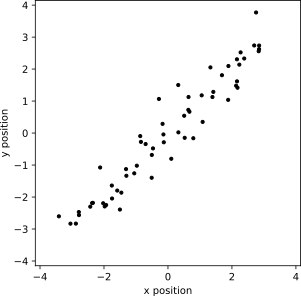
\includegraphics[width=0.8\linewidth]{figs/some_nice_data_org}
	\caption{Randomly generated sample data. The data lies along a line with slope $1$ and has mean $\mathbf{0}$.}
	\label{fig:some_nice_data}
\end{figure}

For larger values of $n$ this gets increasingly difficult\footnote{For higher dimensionality we have to use some projection. Depending on the chosen projection the interpretation changes making it difficult to interpret the resulting image.}. PCA tries to solve this problem by transforming the data in such a way that the most interesting features are in the first few axis of the transformed $m$ dimensional space. This makes it easy to look at a low dimension representation of the data, without loosing much information.

An example of PCA being applied to the data from figure~\ref{fig:some_nice_data} can be seen in figure~\ref{fig:pca_example}. In the top figure the normed data and the direction of the new axis (called principal components) in relation to the two original axis are shown. The bottom figure depicts the transformed data. One can see that the variance is maximal in the first principal component.

\begin{figure}
	\centering
	\begin{subfigure}{0.8\linewidth}
		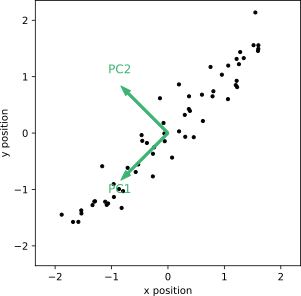
\includegraphics[width=\textwidth]{figs/some_nice_data_pc}
		\caption{Normed data (mean is zero and variance is one) and direction of the two principal components (PC1, PC2) in relation to the x and y position.}
		\label{fig:some_nice_data_pc}
	\end{subfigure}
	\hfill
	\begin{subfigure}{0.8\linewidth}
		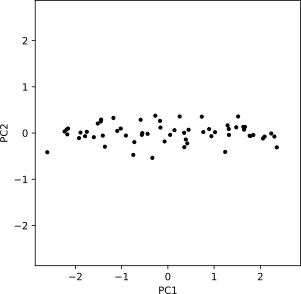
\includegraphics[width=\textwidth]{figs/some_nice_data_pca}
		\caption{The data after being transformed by PCA. The variance along the first principal component (PC1) axis is maximal, therefore the data is spread out most along this axis.}
		\label{fig:some_nice_data_pca}
	\end{subfigure}
	
	\caption{Example application of PCA.}
	\label{fig:pca_example}
\end{figure}

Now we derive the ideas of PCA, as well as the mathematics behind it. First we formulate a goal and define some assumptions.

We assume that the most interesting features are those that have a large variance\footnote{This assumption can be false. For data where the noise has a larger variance than the feature we are trying to observe, PCA fails because this assumption is not met.}. Our goal is to find a transformation into new coordinates such that:
\begin{itemize}
	\item the variance in the each axis is as large as possible.
	\item the axis are all orthogonal to each other.
	\item the axis are sorted (descending) by the variance in the axis.
\end{itemize}

From this we gather that another assumption is, that the axis are orthogonal. Lastly we are only concerned with linear dependent features in the data. Some example cases in which PCA fails are shown in figure~\ref{fig:pca_fails}.

\begin{figure}
	\centering
	\begin{subfigure}{0.8\linewidth}
		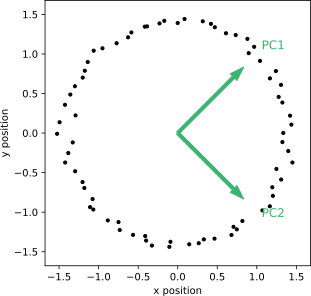
\includegraphics[width=\textwidth]{figs/pca_fails_nonlinear}
		\caption{Clearly the relationship in this figure is non-linear. PCA can not describe circular dependencies, as shown in this data.}
		\label{fig:pca_fails_nonlinear}
	\end{subfigure}
	\hfill
	\begin{subfigure}{0.8\linewidth}
		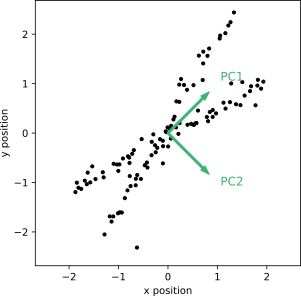
\includegraphics[width=\textwidth]{figs/pca_fails_nonorthogonal}
		\caption{The two main axis along which the data is aligned are not orthogonal to each other. PCA always outputs orthogonal principal components, therefore it fails in this example.}
		\label{fig:pca_fails_nonorthogonal}
	\end{subfigure}
	
	\caption{Examples in which some of the assumptions of PCA are not valid. The results are sub-optimal.}
	\label{fig:pca_fails}
\end{figure}


\newpage
One way to achieve the goal is as follows:
\begin{enumerate}
	\item Find the direction which maximizes the variance.
	\item Save this direction as the next axis.
	\item Determine the subspace that is orthogonal to all axis we found so far.
	\item If the subspace is non-trivial start at the first step again.
	\item If the subspace is trivial we have found all axis.
\end{enumerate}

While this algorithm shows us what conceptually has to be done, we do not know how to compute the axis yet. We will now investigate this problem using the mathematical concepts from section~\ref{chapter:mathematical_basics}. This will lead us to an algorithm in which all axis can be computed simultaneously.

Let $\mathbf{X} \in \mathbbm{R}^{m\times n}$ be the data matrix. We want to find some orthonormal matrix $\mathbf{P}$ such that $\mathbf{Y}:=\mathbf{PX}$ has a diagonal covariance matrix $\mathbf{C}_{\mathbf{Y}}$.

\begin{align*}
	\mathbf{C}_{\mathbf{Y}} = \frac{1}{n}\mathbf{YY}^T = \frac{1}{n}(\mathbf{PX})(\mathbf{PX})^T = \frac{1}{n}\mathbf{PX}\mathbf{X}^T\mathbf{P}^T =\\
	= \mathbf{P}(\frac{1}{n}\mathbf{X}\mathbf{X}^T)\mathbf{P}^T = \mathbf{P}\mathbf{C}_\mathbf{X}\mathbf{P}^T
\end{align*}

The covariance matrix $\mathbf{C}_\mathbf{X}$ is symmetric and therefore has a decomposition into an orthogonal matrix of eigenvectors $\mathbf{V}$ and a diagonal matrix of eigenvalues $\mathbf{D}$. We choose $\mathbf{P}=\mathbf{V}^T$. From lemma~\ref{lem:inverse_is_transpose} it follows that $\mathbf{V}^{-1} = \mathbf{V}^T$.

\begin{align*}
	\mathbf{P}\mathbf{C}_\mathbf{X}\mathbf{P}^T = \mathbf{P}(\mathbf{VDV}^{-1})\mathbf{P}^T = \mathbf{P}(\mathbf{VDV}^{T})\mathbf{P}^T =\\
	\mathbf{P}(\mathbf{P}^T\mathbf{DP})\mathbf{P}^T = (\mathbf{P}\mathbf{P}^T)\mathbf{D}(\mathbf{P}\mathbf{P}^T) =\\
	(\mathbf{P}\mathbf{P}^{-1})\mathbf{D}(\mathbf{P}\mathbf{P}^{-1}) = \mathbf{D}
\end{align*}

In summary $\mathbf{Y}$ has a diagonal covariance matrix if we choose $\mathbf{Y} = \mathbf{V}^T\mathbf{X}$, where $\mathbf{V}$ is the matrix of eigenvectors of $\mathbf{C}_\mathbf{X}$. The eigenvectors are the principal components and the eigenvalues are the variance in each new axis.

As pseudo code we get the program from algorithm~\ref{alg:pca} for calculating the PCA.

\begin{algorithm}
	\caption{Principal Component Analysis}\label{alg:pca}
	\begin{algorithmic}
		\Require matrix $X \in \mathbbm{R}^{m\times n}$
		\State Normalize each row in the matrix $X$
		\State Calculate the covariance matrix $C_{X}$
		\State Calculate the eigenvalues and eigenvectors of $C_{X}$
		\State Sort the eigenvalues
		\State Return sorted eigenvalues and corresponding eigenvectors
	\end{algorithmic}
\end{algorithm}

What happens if we skip the step in which we normalize each row in the matrix? A big variance is interpreted by the PCA algorithm as much information, thus the variance of the variables have an impact on how ''important'' the variable is deemed. As we do not want to prioritize certain variables we avoid this behavior by normalizing the data beforehand.

\chapter{Methodology}
\label{chapter:methodology}
\chapter{\color{change} Supporting Methods: FFT and KNN \color{black}}
\label{chapter:methodology}

For the main algorithm of this work from section~\ref{chapter:data_and_algorithm} a two other methods will be used. As they are not the focus of this work we only give a short overview \color{change} in this chapter. \color{black}

\section{Fourier Transformation}
\label{sec:fourier_transformation}

Many applications are concerned with cyclic temporal data. \color{change} Examples are sound waves, seismic data, oscillations of a skyscraper in strong wind or EEG data. \color{black} This data can be represented as a function of amplitude over time. Most of the time we are not interested in the amplitude at a specific point in time, as a temporal shift would represent very similar information. Such a shift is demonstrated in figure~\ref{fig:tempoal_shift}.

\begin{figure}
	\centering
	
	\begin{subfigure}[b]{\textwidth}
		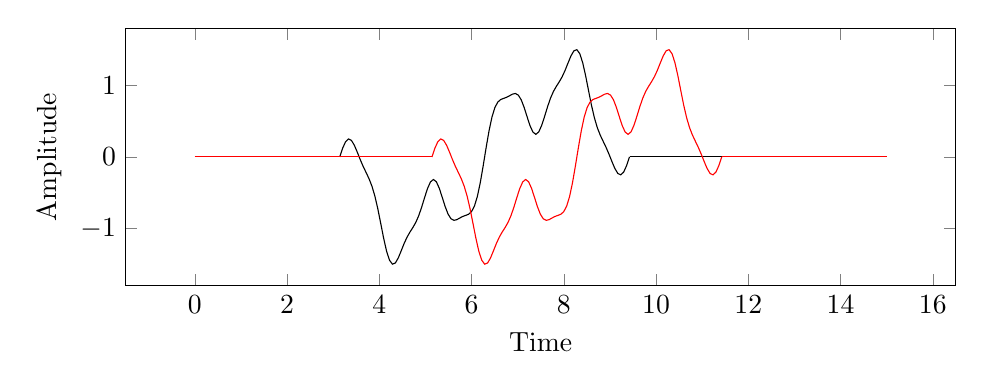
\begin{tikzpicture}
			\begin{axis}[xlabel=Time, ylabel=Amplitude, width=\textwidth, height=0.4\textwidth]
				\addplot+ [domain=0:pi, samples=100, no marks, color=black, style=solid]{0};
				\addplot+ [domain=pi:3*pi, samples=100, no marks, color=black, style=solid]{sin(deg(x)) + 0.5*sin(deg(4*x)) + 0.1*sin(deg(10*x))};
				\addplot+ [domain=3*pi:15, samples=100, no marks, color=black, style=solid]{0};
				
				\addplot+ [domain=0:pi+2, samples=100, no marks, color=red, style=solid]{0};
				\addplot+ [domain=pi+2:3*pi+2, samples=100, no marks, color=red, style=solid]{sin(deg(x-2)) + 0.5*sin(deg(4*(x-2))) + 0.1*sin(deg(10*(x-2)))};section
				\addplot+ [domain=3*pi+2:15, samples=100, no marks, color=red, style=solid]{0};
			\end{axis}
		\end{tikzpicture}
	\end{subfigure}
	
	\caption{Two signals that differ by a temporal shift.}
	\label{fig:tempoal_shift}
\end{figure}

As the function of sound waves or EEG data is cyclic we might be interested in a decomposition into simple cyclic function, such as sine. We can then analyze the most prominent frequencies and their respective amplitudes. This gives a representation of the data, that can be easier to interpret.

We describe one approach to achieve this representation as a weighted sum of sinoid functions, called Fast Fourier Transformation (FFT), in algorithm~\ref{alg:fft}.
Figure~\ref{fig:example_fft} shows an example input and output of the FFT algorithm.

\begin{algorithm}
	\caption{Fast Fourier Transformation}\label{alg:fft}
	\begin{algorithmic}
		\Function{FFT}{$x$, $N$, $s$}
			\If{$N$ = $1$}
				\State $X_0 \gets x_0$
			\Else
				\State $X_{0, ..., N/2-1} \gets FFT(x, N/2, 2s)$
				\State $X_{N/2, ..., N-1} \gets FFT(x+s, N/2, 2s)$
				\For{$k=0$ to $N/2-1$}
					\State $p \gets X_k$
					\State $q \gets \exp(-2\pi i/N k) X_{k+N/2}$
					\State $X_k \gets p + q$
					\State $X_{k+N/2} \gets p - q$
				\EndFor
			\EndIf
			\State \Return $X_{0, ..., N-1}$
		\EndFunction
	\end{algorithmic}
\end{algorithm}

\begin{figure}
	\centering
	
	\begin{subfigure}[b]{\textwidth}
		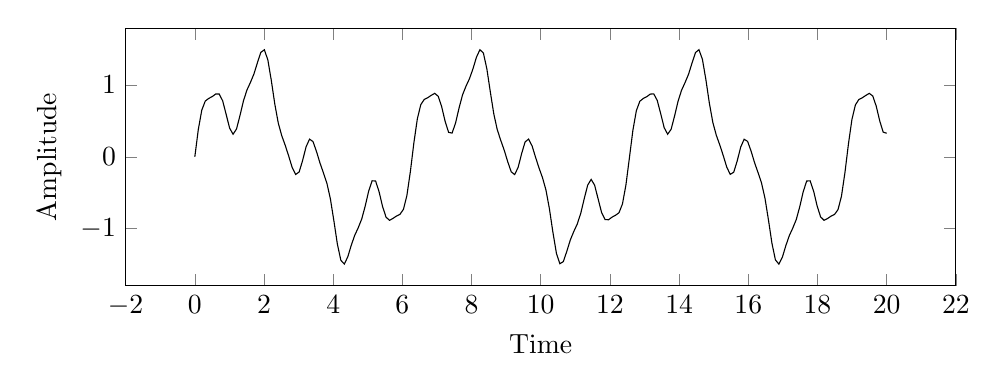
\begin{tikzpicture}
			\begin{axis}[xlabel=Time, ylabel=Amplitude, width=\textwidth, height=0.4\textwidth]
				\addplot+ [domain=0:20, samples=200, no marks, color=black]{sin(deg(x)) + 0.5*sin(deg(4*x)) + 0.1*sin(deg(10*x))};
			\end{axis}
		\end{tikzpicture}
	\end{subfigure}
	\vskip\baselineskip
	\begin{subfigure}[b]{\textwidth}
		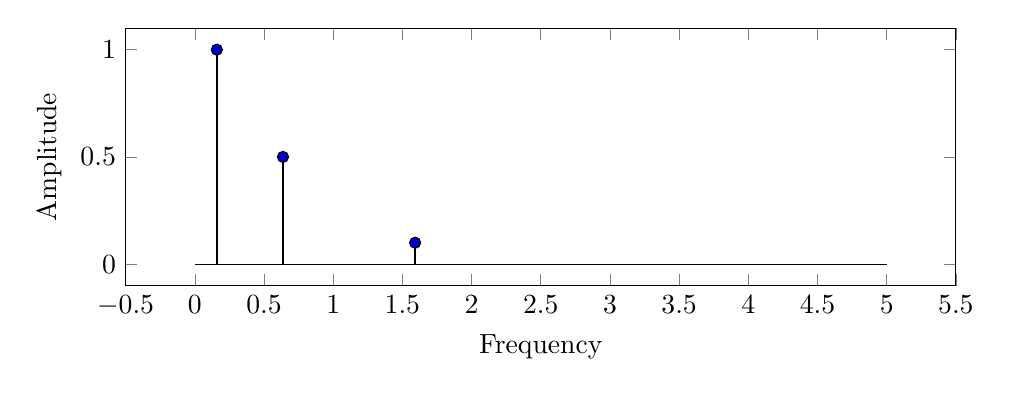
\begin{tikzpicture}
			\begin{axis}[xlabel=Frequency, ylabel=Amplitude, width=\textwidth, height=0.4\textwidth]
				\addplot+ [mark=*, only marks, ybar, bar width=0.5pt, color=black] coordinates {
					(0.159, 1)
					(0.637, 0.5)
					(1.592, 0.1)
				};
				\addplot+ [domain=0:5, samples=100, no marks, color=black]{0};
			\end{axis}
		\end{tikzpicture}
	\end{subfigure}
	
	\caption{A signal composed of different sinoid functions and the corresponding FFT output.}
	\label{fig:example_fft}
\end{figure}

\newpage

\section{Classification}
\label{sec:classification}

As the classification algorithm is not the main focus of this work, we decided to go with a simple one.

The objective of classification is to find assignments between data points and categories. In our context we are interested in finding an assignment which closely matches some already categorized data. One simple approach to this problem is the $k$-nearest-neighbors algorithm (KNN).

For data that can be represented in $\mathbbm{R}^m$ and $l$ categories the pseudo code is shown in algorithm~\ref{alg:k_nearest_neighbors}.

\begin{algorithm}
	\caption{$k$ Nearest Neighbors}\label{alg:k_nearest_neighbors}
	\begin{algorithmic}
		\Require data points $(p_i)_{i \in \mathbbm{N}} \in \mathbbm{R}^{m}$, categories $(c_i)_{i \in \mathbbm{N}}, c_i \in \{0, 1, ..., l\} \forall i \in \mathbbm{N}$,
		
		point $x \in \mathbbm{R}^{m}$, $k \in \mathbbm{N}$
		\State Calculate the distance between each point $p_i$ and $x$
		\State Take the $k$ data points with the smallest distance to $x$
		\State \Return the category that most of the $k$ points are assigned
	\end{algorithmic}
\end{algorithm}

If there are significantly more data points in a certain category KNN can be dominated by these categories. As there are more points in the category, they are statistically more common in the $k$ nearest, which leads to $k$-nearest-neighbor giving bad results.

Variations of KNN are achieved by applying a weight to the data points. The weight can depend on the distance between the points.

This algorithm is slow for big datasets as for each point the distance to $x$ has to be calculated. One possibility to reduce calculation time is to partition the space into smaller chunks. Then the loop only has to be over data points lying in the same or close chunks as the point we are interested in.

Figure~\ref{fig:k_nearest_neighbors} shows a graphical representation of the algorithm for points in $\mathbbm{R}^2$ and ${k=10}$.

\begin{figure}
	\centering
	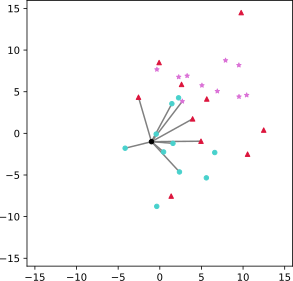
\includegraphics[width=0.45\linewidth]{figs/k_nearest_neighbors}
	\caption{Data points in three categories are given. The black point is classified as a blue, circular point by the k-nearest-neighbors algorithm for $k=10$.}
	\label{fig:k_nearest_neighbors}
\end{figure}

\chapter{Data and Algorithm}
\label{chapter:data_and_algorithm}
\chapter{Data and Algorithm}
\label{chapter:data_and_algorithm}

This chapter describes the CAP Sleep Database used and the algorithm implemented. The algorithm uses FFT, PCA and k-nearest neighbor to estimate the sleep stage from a recorded EEG signal.

\section{Data}
\label{sec:data}

We use the CAP Sleep Database\cite{Terzano2001}\cite{Goldberger2000} which provides 16 recordings of patients without pathology. Two of these recordings have corrupted files and one did not have the data points used for this analysis and thus could not be analyzed. The table~\ref{tab:meta_data_of_recordings} shows some meta data of the recordings.

\begin{table}
	\centering
	\begin{tabular}{c|c|c|c|c|c}
		File Name & Age & Gender & Length of Recording & Channel Name & Sampling Frequency \\
		\hline
		n1  & 37 & F & 577 minutes & C4-A1  & 512 Hz \\
		n2  & 34 & M & 735 minutes & C4-A1  & 512 Hz \\
		n3  & 35 & F & 551 minutes & C4-A1  & 512 Hz \\
		n4  & 25 & F & 596 minutes & C4-A1  & 200 Hz \\
		n5  & 35 & F & 524 minutes & C4-A1  & 512 Hz \\
		n6  & 31 & M & 527 minutes & C3-A2  & 128 Hz \\
		n7  & 31 & M & 492 minutes & C3-A2  & 128 Hz \\
		n8  & 42 & F & 501 minutes & C3-A2  & 200 Hz \\
		n9  & 31 & M & 532 minutes & C3-A2  & 128 Hz \\
		n10 & 23 & M & 490 minutes & C4-A1  & 512 Hz \\
		n11 & 28 & F & 527 minutes & C4-A1  & 512 Hz \\
		n12 & 29 & M & 495 minutes & C3-A2  & 100 Hz \\
		n16 & 41 & F & 513 minutes & C4-A1  & 100 Hz \\
	\end{tabular}
	\caption{Meta data of the 13 recordings from the CAP Sleep Database.}
	\label{tab:meta_data_of_recordings}
\end{table}

The given dataset describes multiple channels of EEG data recorded during sleep. We are interested in the channels recording activity in the central area, as these are the two channels most of the recordings shared. The figure~\ref{fig:head_placement} shows where the sensors were placed.

\begin{figure}
	\centering
	\includegraphics[width=0.7\linewidth]{figs/head_placement}
	\caption{Scheme of sensor placement in recordings of EEG data.}
	\label{fig:head_placement}
\end{figure}

The data was recorded in different frequencies. To reduce data size and standardize all channels we resample to 200 Hz.

Very low and very high frequencies often stem from other sources, such as the measurement equipment, breathing of the patients or measuring inaccuracies. To get rid of these noises we apply a low pass filter of 30 Hz and a high pass filter of 0.5 Hz.

\section{Algorithm}
\label{sec:algorithm}

We now describe the general structure of the algorithm from reading the data files to the clustering.

First we split the recorded data into 30 second sections. For each of these sections we get the data as a function of amplitude over time. An example segment is shown in the upper figure of~\ref{fig:example_30s_segment}. We apply a Fourier transformation as described in section~\ref{sec:fourier_transformation} and get a function of amplitude over frequency. This gives a frequency based representation of the data. As the sleep stages are characterized by different frequencies and amplitudes, as described in section~\ref{sec:eeg_data_and_sleep_stages}, this will help us distinguishing them. The output of such an FFT can be seen in the lower figure of~\ref{fig:example_30s_segment}. The pseudo code for this processing is described in algorithm~\ref{alg:process_eeg_data}.

\begin{algorithm}
	\caption{EEG data processing}\label{alg:process_eeg_data}
	\begin{algorithmic}
		\For{each patient}
		\State Read EEG data from file
		\State Apply a 30 Hz low pass and a 0.5 Hz high pass filter
		\State Resample with frequency 200 Hz
		\State Get one of the channels C4-A1 or C3-A2 (in this order)
		\State Section out the part of data where the patient is asleep
		\For{each 30 second segment of the data}
		\State Do a Fourier transformation (FFT)
		\EndFor
		\State Save all the outputs from the FFT to the patients file
		\EndFor
	\end{algorithmic}
\end{algorithm}


\begin{figure}
	\centering	
	\begin{subfigure}[b]{\textwidth}
		\begin{tikzpicture}
			\begin{axis}[xlabel=Time (seconds), ylabel=Amplitude, width=\textwidth, height=0.3\textwidth]
				\addplot+ [no marks, color=black] table[col sep=comma] {figs/example_30s_segment1.csv};
			\end{axis}
		\end{tikzpicture}
	\end{subfigure}
	\vskip\baselineskip
	\begin{subfigure}[b]{\textwidth}
		\begin{tikzpicture}
			\begin{axis}[xlabel=Frequency (Hz), ylabel=Amplitude, width=\textwidth, height=0.3\textwidth]
				\addplot+ [no marks, color=black] table[col sep=comma] {figs/example_30s_segment2.csv};
			\end{axis}
		\end{tikzpicture}
	\end{subfigure}
	
	
	\caption{A 30 second segment of the data. The top shows the recorded signal of the EEG. The bottom shows the output of the Fourier transformation.}
	\label{fig:example_30s_segment}
\end{figure}

We now have high dimensional data points, as each 30 second segment is represented by the amplitudes for each of the distinct frequencies output by the FFT. Before we can start searching for cluster in the data we want to find a lower dimensional representation. This is were PCA can be used. From the output of algorithm~\ref{alg:pca_of_eeg_data} we get principal components, which reveal the frequencies were the most variance is shown. Under our assumptions this variation is caused by the different sleep stages each recording goes through. We show a visual representation of the data in the first three principal components in figure~\ref{fig:pca_output_3d}.

\begin{algorithm}
	\caption{Apply PCA to the EEG data}\label{alg:pca_of_eeg_data}
	\begin{algorithmic}
		\For{each patient}
			\State Read FFT output from patients file
			\State Read the sleep stages from another file
		\EndFor
		\State Concatenate FFT data of all patients
		\State Concatenate sleep stages of all patients
		\State Do PCA on the combined FFT data
		\State Transform data according to the principal components from the PCA
		\State Visualize the data in the first three axis, with the color corresponding to the sleep stage
	\end{algorithmic}
\end{algorithm}

\begin{figure}
	\centering
	\includegraphics[width=\linewidth]{figs/pca_output_3d}
	\caption{Three dimensional representation of the data. Each 30 second segment is represented by a dot in the color corresponding to the sleep stage this segment is assigned to. Awake is represented by red, orange is REM, yellow is S1, green S2 and blue S3.}
	\label{fig:pca_output_3d}
\end{figure}

If we have a new recording and want to know the sleep stages we have to follow similar steps. First the recording has to be split into 30 second segments. These have to be transformed by a FFT. The output can be converted to the PCA basis by multiplying with the matrix of principal components. Lastly we can get a estimate of the sleep stage by using the k nearest neighbor algorithm. The pseudo code is shown in algorithm~\ref{alg:gues_sleep_stage}.

\begin{algorithm}
	\caption{Get estimate for sleep stage}\label{alg:gues_sleep_stage}
	\begin{algorithmic}
		\Require{EEG recording of sleep}
		\For{each 30s segment}
			\State Do FFT on the segment
			\State Multiply FFT output by principal component matrix
			\State Reduce dimensions
			\State Do k nearest neighbor
			\State Save the result of k nearest neighbor
		\EndFor
		\State \Return results of k nearest neighbor
	\end{algorithmic}
\end{algorithm}


\chapter{Results}
\label{chapter:results}

\chapter{Conclusion}
\label{chapter:conclusion}



\bibliographystyle{alpha} 
%\bibliographystyle{abbrv}
\bibliography{literature.bib}

\end{document}
